\documentclass[a4paper,12pt,titlpage]{posobie}
\usepackage[utf8]{inputenc}
\usepackage[english,russian]{babel}
\usepackage{indentfirst}
\usepackage{graphicx}
\usepackage{multicol}

\usepackage{listings}

\lstset{postbreak=\space, 
        breakindent=5pt, 
        breaklines=true, 
        extendedchars=true, 
        inputencoding=cp1251,
        language=Matlab,
        basicstyle=\scriptsize,
        showlines=true
        }
\lstdefinestyle{numbers}
    {numbers=left, stepnumber=1, numberstyle=\tiny, numbersep=10pt}


% Настройки шрифтов

%\renewcommand{\rmdefault}{ftm}
%\renewcommand\normalsize{\fontsize{14}{19} \selectfont}
%\renewcommand\footnotesize{\fontsize{12}{12} \selectfont}
%\renewcommand\small{\fontsize{12}{14} \selectfont}

\def\"{{\char'042}}

% Окружения

\newcommand{\MarkDot}{{$\bullet$}} %% Маркер списка с точками

% Список с маркерами точками

\newenvironment{dotlist}%
    {\begin{list}{\MarkDot}{\partopsep=0mm\itemsep=0mm\topsep=0mm\parsep=0mm\partopsep=0mm\parskip=0mm}}%
    {\end{list}}


\newenvironment{condlg}%
   {\endgraf\verbatim\tt\parindent=0pt}%
   {\endverbatim}

% Нумерованный список

\newenvironment{enum}%
{\begin{list}{\arabic{enumi}.~}{\usecounter{enumi}\partopsep=0mm\itemsep=0mm\topsep=0mm\parsep=0mm\partopsep=0mm\parskip=0mm}}%
   {\end{list}}

% Список с черточкой

\newenvironment{dflist}%
    {\begin{list}{\bfseries--}{\partopsep=0mm\itemsep=0mm\topsep=0mm\parsep=0mm\partopsep=0mm\parskip=0mm}}%
{\end{list}}

\newenvironment{qlist}%
    {\small\begin{enumerate}\itemsep=0mm\topsep=0mm\parsep=0mm\partopsep=0mm\parskip=0mm\vspace{-.3mm}}%
    {\end{enumerate}\vspace{-.5mm}}

\setcounter{secnumdepth}{3} %% Глубина нумерации разделов в тексте
\setcounter{tocdepth}{3}


\makeatletter
\title{Исследование}
\author{Зубарев\,П.\,С., Свириденко\,С.\,В.}
\date{лето 2007}

\renewcommand{\l@section}{\@dottedtocline{1}{10mm}{7mm}}
\renewcommand{\l@subsection}{\@dottedtocline{2}{1.6cm}{9.5mm}}
\renewcommand{\l@subsubsection}{\@dottedtocline{3}{2.6cm}{13mm}}

\renewcommand{\section}{\@startsection{section}{1}{0.0cm}{0.5cm}{0.1cm}%
             {\fontsize{16}{16}\bf\selectfont }}

\renewcommand{\subsection}{\@startsection{subsection}{2}{0.0cm}{0.3cm}{0.1cm}%
             {\fontsize{14}{16}\bf\selectfont }}

\renewcommand{\subsubsection}{\@startsection{subsubsection}{3}{0.0cm}{0.2cm}{0.1cm}%
    {\fontsize{16}{16}\it\selectfont }}

\renewcommand{\paragraph}{\@startsection{paragraph}{4}{12mm}{0.0cm}{-0.20cm}%
    {\bf\selectfont}}

\renewcommand{\thesection}{\arabic{section}.}
\renewcommand{\thesubsection}{\arabic{section}.\arabic{subsection}.}
\renewcommand{\thesubsubsection}{\thesubsection\arabic{subsubsection}.}
\renewcommand{\theparagraph}{\thesubsubsection\arabic{paragraph}.}
\renewcommand{\thesubparagraph}{\theparagraph\arabic{subparagraph}.}
\renewcommand{\thetable}{\thesection\arabic{table}}
\renewcommand{\thefigure}{\arabic{figure}}
\renewcommand{\@seccntformat}[1]{{\csname the#1\endcsname}\hspace{0.1cm}}

%\renewcommand\Bibname{\@startsection{section}{1}{0.0cm}{0.5cm}{0.1cm}{\fontsize{16}{16}\bf\selectfont }Cписок литературы}

\sloppy

  \textwidth=16.5cm
  \oddsidemargin=0in
  \evensidemargin=0in
  \textheight=259mm
  \topmargin=-1cm
  \hoffset=-0.7cm
  \voffset=-1.5cm
  \parindent=12mm
  \pagebreak

\begin{document}
%%%------------- титульный лист ---------------------- 
 
 \thispagestyle{empty} 
 \begin {center} 
 Министерство образования и науки Российской Федерации 
 
 Федеральное агентство по образованию 
 \vspace{0.3cm} 

 Санкт-Петербургский Государственный Электротехнический Университет 

 \vspace{0.3cm} 
 
 Факультет компьютерных технологий и информатики
 
 Кафедра математического обеспечения ЭВМ
 
 
 \vspace {100mm} 
 
 {\Large \bf Исследование и улучшение метода гистограмм} 
 

 \vspace {5mm} 
 курсовая  работа


 \vspace {25mm} 
 

 {\raggedleft 
 

 \vspace {10mm}


 Работу выполнили студенты гр. 3305: 

 Зубарев П.С.\\

 Свириденко С.B. 

   
 
 \vspace {50mm} 
 
 Санкт-Петербург 2007} 
 \end {center} 
 
 %%% ------------------ титульный лист, конец ------------------
\tableofcontents\thispagestyle{empty}

\pagebreak

\section*{Введение}
\addcontentsline{toc}{section}{Введение}


    Многие из нас ассоциируют биометрию или с идентификационными картами, или с контролем 
доступа на основе считывания отпечатков пальцев, или же с системами распознавания черт лица, 
используемыми при видео наблюдении, однако редко кто задумывался о действительном значении биометрии. 
Согласно определению, которое дает Оксфордский толковый словарь, биометрия --- это <<наука приложения 
статистических методов к биологическим проявлениям>>.

    Цель биометрических технологий --- создать механизм однозначной идентификации объекта, 
используя статистические измерения определенных характеристик или поведения этого объекта.
Такая уникальная биометрическая информация может быть сохранена в электронном виде, а затем 
извлечена из базы данных и использована для идентификации. 

    Опознание человека по лицу сегодня используется как метод идентификации буквально сплошь
и рядом, однако многое при этом зависит от человека --- например, от охранника, который
должен определить, соответствуют ли черты лица фотографии в пропуске. Поистине переворотом стала техника сканирования
лица, которая в биометрической индустрии сейчас занимает второе место после сканирования отпечатков пальцев.

    Биометрическое опознание лица, использующее специально разработанное программное обеспечение, 
избавляет от необходимости присутствия человека при проведении идентификации. [2]


\section*{Постановка задачи}
\addcontentsline{toc}{section}{Постановка задачи}

Методы опознавания основаны на преобразовании черт конкретного лица в алгоритмическую модель, которая сравнивается или
с фотографии на пропуске, или с содержимым базы фотографических данных. Проще говоря, для каждого
образа создается уникальный <<пароль>>, содержащий характеристики черт лица. По лицу человека 
можно узнать его историю, симпатии и антипатии, болезни, эмоциональное состояние, 
чувства и намерения по отношению к окружающим. Всё это представляет особый интерес для автоматического
распознавания лиц (например, для выявления потенциальных преступников).
    
    Наиболее часто на практике распознавания лиц человека применяют яркостные методы, как способ представления 
характеристик лица человека. Среди причин применения яркостных методов можно выделить две основные.

    Во-первых, яркостные признаки по своей сути представляют любое цифровое изображение и  
не изменяются при плоских поворотах и изменении размеров.
   
    Во-вторых, яркостные признаки позволяют выделить области с резким перепадом яркости, которые могут
соответствовать определенным областям лица. Сами перепады будут находиться на границах этих областей.[1]

    Процесс распознавания можно определить следующим образом. Пусть есть несколько разных изображений лиц 
или образов заданного класса\footnote{изображения одного и того же объекта относятся к одному классу}, которых находятся в базе 
данных. Каждый такой образ можно представить как эталон. В процессе распознавания на вход системе поступает новый образ, 
который необходимо идентифицировать. Для этого необходимо проверить принадлежность этого образа базе данных: вычисляя
либо некоторую меру подобия между новым образом и каждым эталоном из базы, либо меру подобия между некоторой характеристикой
нового образа и совместной характеристикой образов в классе.[1]

     Новый образ будет принадлежать тому классу, мера подобия с которым будет наивысшей. Однако в случае если на вход системе
поступит изображение для которого нет эталона в базе, будет произведена неверная идентификация. Для того чтобы отсеять часть неверных 
решений, можно ввести минимальный порог подобия. В таком случае если наивысшая мера подобия между входным образом и всеми эталонами
получилась меньше этого порога, то можно сказать, что изображение не было идентифицировано. 

Таким образом весь процесс распознавания можно разложить на следующие этапы:
\begin{dotlist}
\item детекция области лица на исходном изображении;
\item экстракция признаков --- представления изображения выделенного лица в форме вектора исходных признаков;
\item селекции некоторых признаков из полного набора или редукции исходного пространства признаков;
\item сравнения признаков нового образа с признаками эталонов;
\item принятие решения о принадлежности этого образа к одному из известных классов.
\end{dotlist}

\section*{Обзор методов борьбы с освещенностью}
\addcontentsline{toc}{section}{Обзор методов борьбы с освещенностью}
     Рассмотрим процесс распознования с более обощенной стороны. У нас на входе есть некий образ, который необходимо идентифицировать.
Результатом идентификации является нахождение или нет этого образа в базе данных системы распознования. Разобъем процесс распознования на 
следующие три шага:
\begin{enum}
\item получение входной информации
\item обработка исходной информации 
\item распознование(идентификация)
\end{enum}

Бороться с освещенностью можно на любом из данных этапов идентификации. Изображение можно изменять на этапе его получения. Например, в 
камеру, снимающую и передающую изображение в систему идентификации можно встроить фотоэлемент, который будет менять диафрагму камеры в 
зависиомсти от текущей освещенности, что позволит получать качественные картинки как прия ярком дневном свете с выставленной маленькой 
диафрагмой, так и ночью --- с большой диафрагмой. Однако такая модификация требует высоко чувствительную фото-матрицу, чтобы сократить 
время получения кадра ночью, так как при маленькой чувствительности фото-матрицы изображения может быть, либо не очень четким(что не сильно
влияет на яркостные признаки), либо совсем смазанным, что может привести к тому, что разные  изображения с близкими яркостями по яркостным
критериям полностью совпадут. Помимо использования камер с изменяемой диафрагмой, возможно решить данную проблему наиболее простым способом:
установить дополнительное освещение в зоне фокуса камеры, уменьшив таким образом внешнее влияние на освещенность.

В случае если система идентификации работает в сложных световых условиях, улучшить ее стойкость к освещенности можно путем применения 
алгоритмов не использующих яркотные признаки. Например, идентификация по отпечатку пальца или по голосу.

\section*{Гистограммный метод}
\addcontentsline{toc}{section}{Гистограммный метод}
     Одним из главных этапов процесса распознования является этап экстракции признаков. Самым простым, но в тоже время
и эффективным методом является гистограммный метод, который заключается в вычислении гистограммы яркости исходного изображения и 
сведения ее значений в вектор исходных (гистограммных) признаков. 


\subsection*{Вычисление гистограммы}
\addcontentsline{toc}{subsection}{Вычисление гистограммы}

    Вычисление одномерной гистограммы яркости исходного изображения и сведение её значений в вектор гистограммных признаков заключается 
в следующем: каждый элемент гисторграммы $H(j)$ определяется количеством пикселей исходного изображения, имеющих значения яркости, равное 
$j=0,1,2 ... 255$. $H(j)$ --- вектор признаков размерностью $256$. Порой работать с таким большим вектором признаков не очень удобно, и имеет 
смысл произвести редукцию признаков к пространству $DIM$. При редукции пространства признаков гистограмма $H(j)$ 
преобразуется к следующему виду:
\[ H(b) = \sum_{j=(b-1)\frac{256}{BIN}}^{b\frac{256}{BIN}} H(j), b = 1,2,...,BIN \]
В случае если исходное изображение и эталонное изображение, имеют различные размеры, то вектор признаков необходимо нормировать:
\[ H_{norm}(b) = \frac{H(B)}{MN}, b = 1,2,..., BIN \],
где $M$, $N$ -- число строк и число столбцов в исходном изображении.[1]

\subsection*{Применение гистограмм}
\addcontentsline{toc}{subsection}{Применение гистограмм}
     
     Большим преимуществом гистограммного метода является его хорошая стойкость к геометрическим преобразованиям исходной 
картинки. Так если даже исходное изображение повернуть то его гистограммы останется прежней. 

\begin{figure}[h]
 \parbox[h]{0.49\textwidth}{\centering
   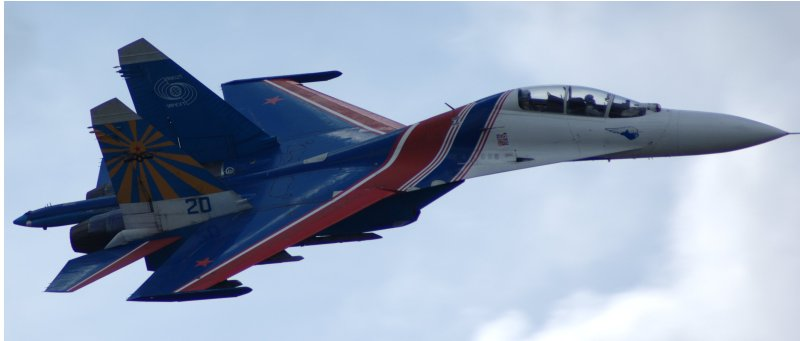
\includegraphics[width=0.49\textwidth]{mig.png}
   \caption{Исходоное изображение}\label{fig:source_img}}
   \hfil\hfil%раздвигаем боксы по горизонтали
   \begin{minipage}[h]{0.49\textwidth}
     \centering
     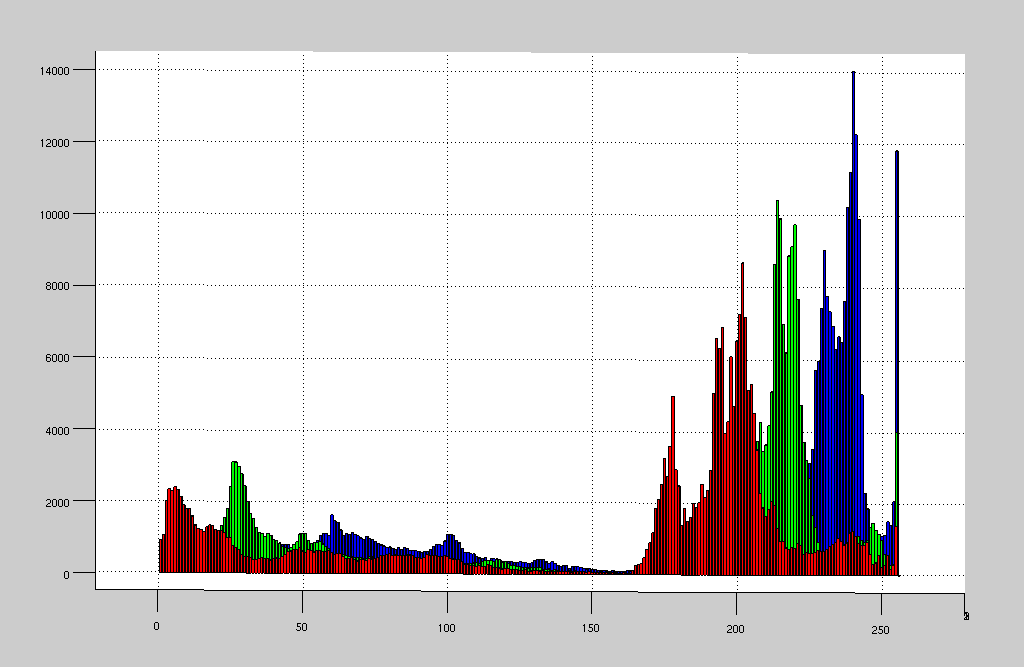
\includegraphics[width=\textwidth]{mig_gist.png}
     \caption{Гистограмма исходного изображения}\label{fig:source_img_gist}
   \end{minipage}
\end{figure}
     На рисунке \ref{fig:source_img} представлено исходное изображение, для которого построена гистограмма (рис. \ref{fig:source_img_gist}). 
\begin{figure}[h]
 \parbox[h]{0.49\textwidth}{\centering
   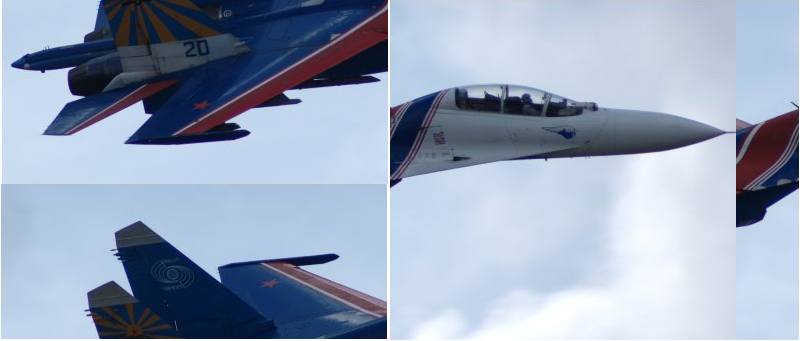
\includegraphics[width=0.49\textwidth]{mig2.png}
   \caption{Измененное изображение}\label{fig:edited_img}}
   \hfil\hfil%раздвигаем боксы по горизонтали
   \begin{minipage}[h]{0.49\textwidth}
     \centering
     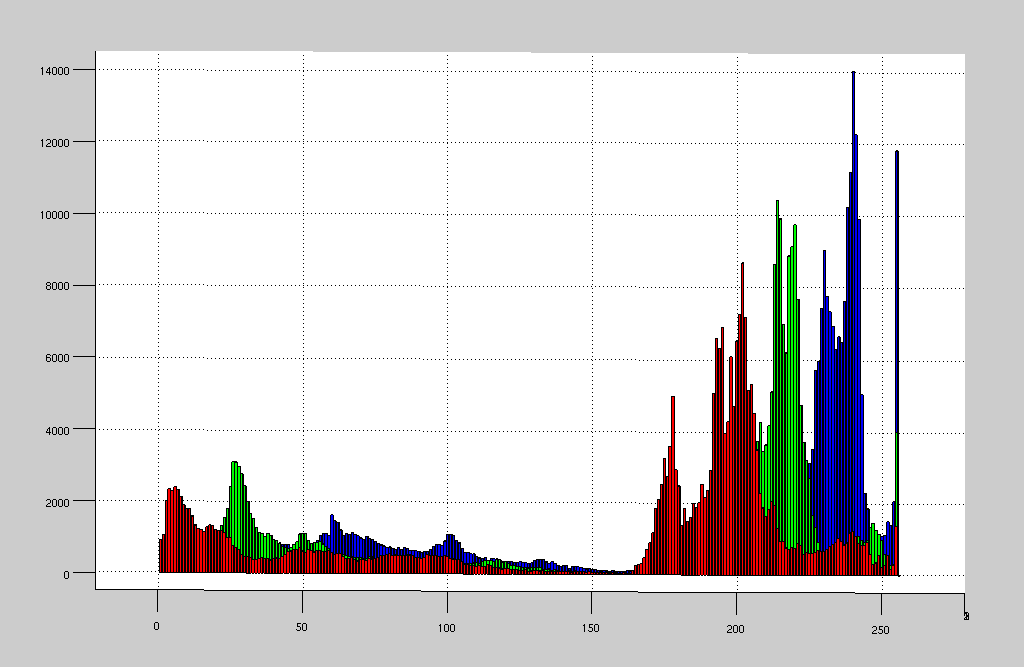
\includegraphics[width=\textwidth]{mig_gist.png}
     \caption{Гистограмма измененного изображения}\label{fig:edited_img_gist}
   \end{minipage}
\end{figure}
     Затем исходное изображение было разрезано на маленькие кусочки, которые были перемешаны внутри изображения (рис. \ref{fig:edited_img}).
Если сравнить гистограммы исходного (рис.\,\ref{fig:source_img_gist}) и измененного (рис.\,\ref{fig:edited_img_gist}) изображения,
то можно обратить внимание, что они совпадают. Это лишний раз
показывает стойкость метода по отношению к геометрическим преобразованиям изображений. Такая особенность гистограмного метода может
быть с легкостью применена в криминалистике. Например, если необходимо идентифицировать личность, когда на входе имеется изображение, 
порезанное на множество маленьких кусочков.
 
     Помимо всего следует отметить некоторые особенности гистограммного метода. Например, чем больше площадь фона вокруг области лица,
тем заметнее различие гистограмм для разных изображений лиц даже при одном и том же фоне. Кроме этого гистограммный метод может
применяться в случае, когда на изображениях фон различается несущественно. 

     Однако следует помнить, что гистограмма --- это яркостная характеристика, поэтому два структурно или текстурно одинаковых, но имеющих
разную яркость изображения будут иметь в общем случае различные по форме гистограммы: от циклического сдвига по отношению друг к другу, до циклического сдвига и искажений на границах.

\subsection*{Модификации метода гистограмм}
\addcontentsline{toc}{subsection}{Модификации метода гистограмм}


    Возможны несколько способов модификации метода гистограмм. Один из видов модификации --- метод, направленный на ускорение вычисления
вектора исходных признаков. В связи с тем что лицо человека достаточно симметрично, то гистограммы левой и правой части лица практически 
идентичны, в результате чего можно воспользоваться только одной половиной лица и построить по нему вектор исходных признаков, который
по качественным показателям не будет отличаться от вектора признаков, построенного по всему лицу. В случае разделении лица по горизонтали 
произойдет существенная потеря данных и в таком случае метод будет неработоспособным. 

    В случае же если у нас в базе данных мало изображений одного класса, с помощью разделения изображения лица 
на две половинки и отражении каждой из половинок относительно оси разделения, можно 
получить два эталонных изображения вместо одного, что может существенно улучшить результат распознавания. 

Цель работы

цель работы состоит в попытке оптимизации гистограммного метода для случая, когда изображения в базе данных и поступающие для распознавания образцы имеют различную степень освещённости.

*картинка с 10 рожами разной освещённости*

\section*{Исследования}
\addcontentsline{toc}{section}{Исследования}


\subsection*{Влияние освещения на гистограмму}
\addcontentsline{toc}{subsection}{Влияние освещения на гистограмму}

Рассмотрим, как меняется гистограмма изображения при осветлении и затемнении:
\begin{figure}[h]
   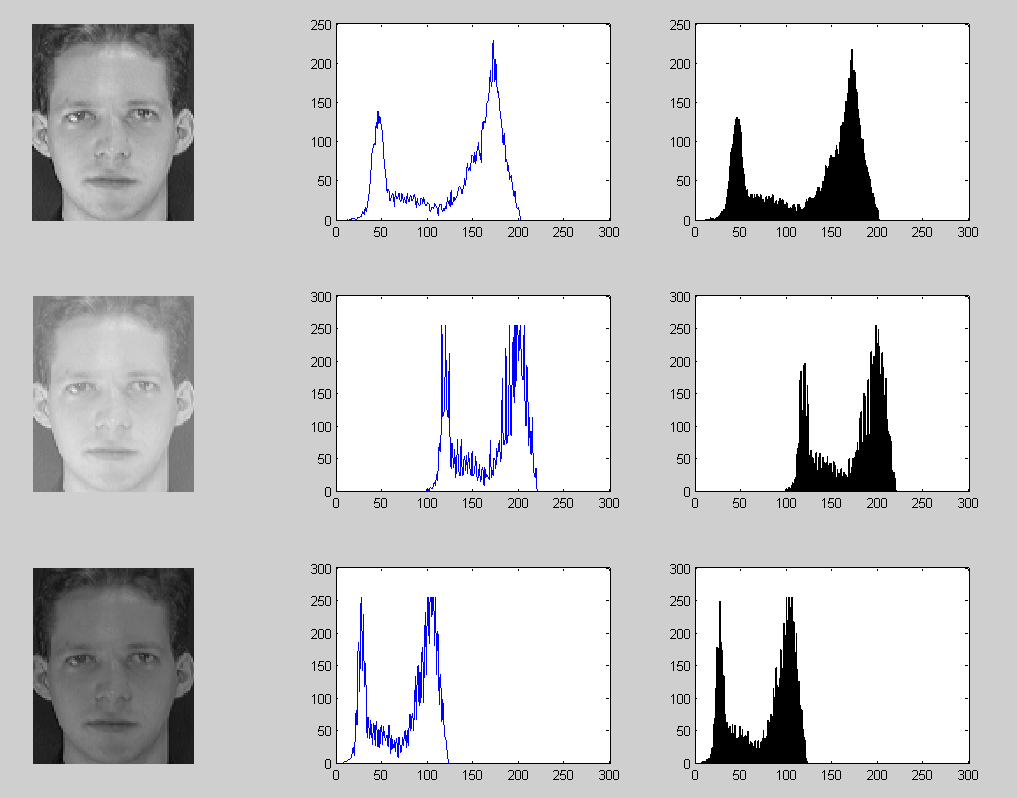
\includegraphics[width=\textwidth]{report/pic_1.png}
   \caption{Влияние осветления/затемнения изображения на характер гистограммы}\label{fig:research_faces}
\end{figure}
В данном случае осветление и затемнение были выполнены в графическом редакторе. Мы видим, что гистограмма не просто 
сдвинулась на определённую величину, но и сжалась по горизонтали. Тем не менее, снимки, сделанные на фотоаппараты и 
камеры, выглядят отлично от представленных образцов. Всё это приводит нас к мысли, что редакторы несколько «облагораживают» картинку. 

Действительно, сравним изображения, осветлённые на одинаковую величину в графическом редакторе и программой на MATLAB:

\begin{figure}[h]
   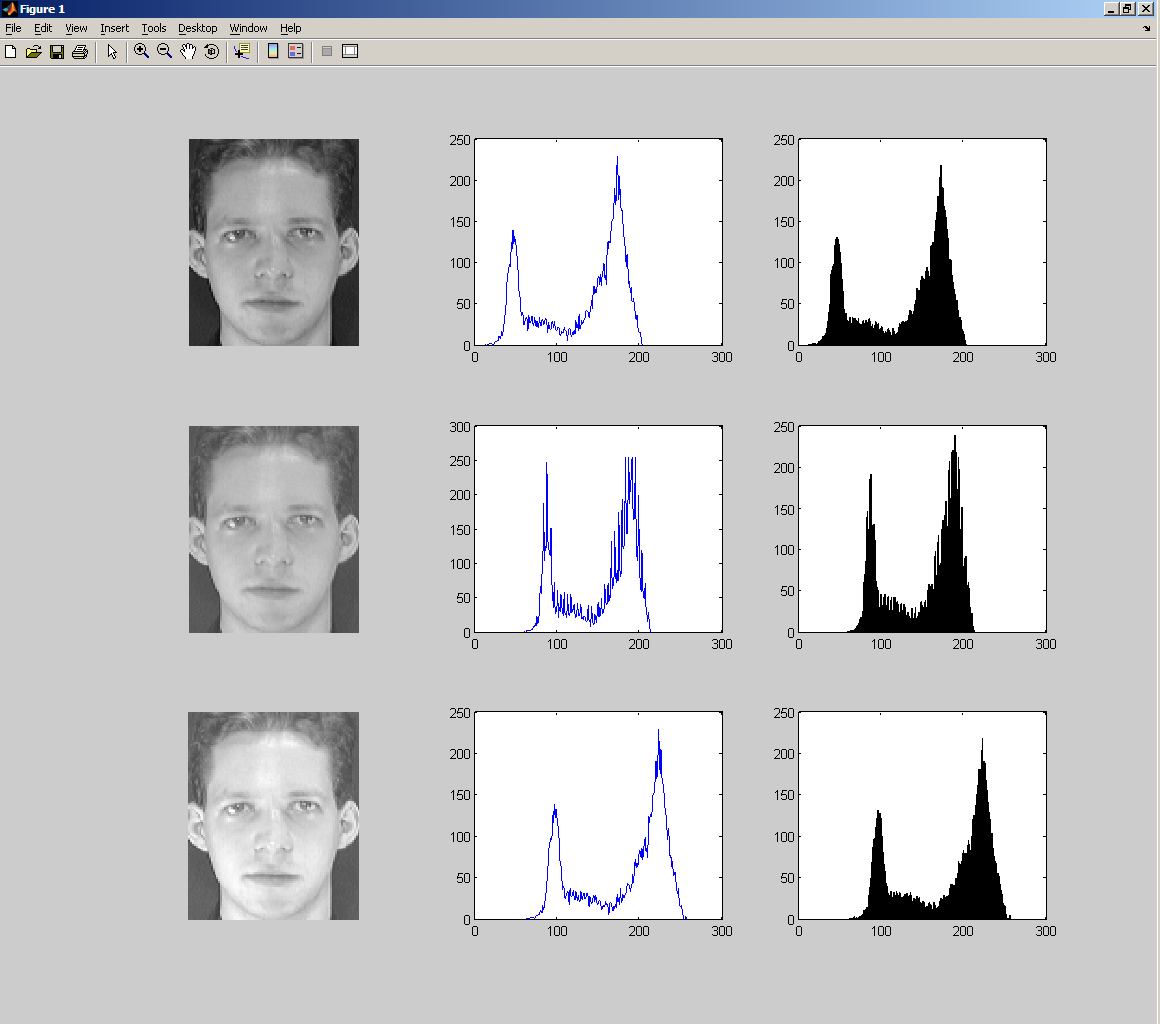
\includegraphics[width=\textwidth]{report/pic_2.png}
   \caption{Осветление +50. Изображения сверху вниз: оригинал, осветление IrfanView, осветление MATLAB}\label{fig:faces_irfan_1}
\end{figure}
Здесь некоторая схожесть улавливается, хотя нижняя картинка больше похожа на то, что мы видели бы в 
реальной жизни. Попробуем сделать ещё большее осветление(рис. \ref{fig:faces_irfan_1}).
\begin{figure}[h]
   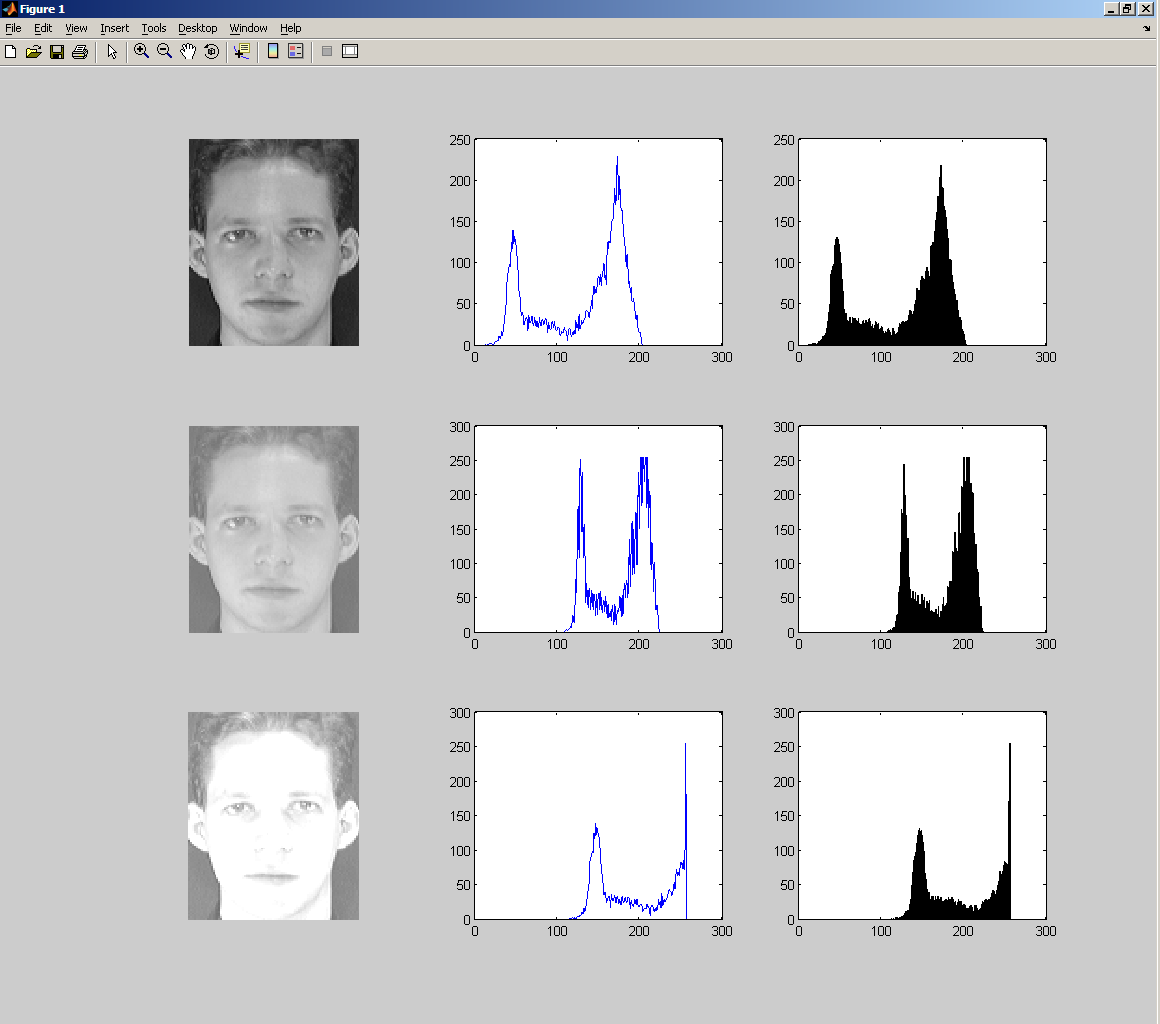
\includegraphics[width=\textwidth]{report/pic_3.png}
   \caption{Осветление +100. Изображения сверху вниз: оригинал, осветление IrfanView, осветление MATLAB}\label{fig:faces_irfan_2}
\end{figure}
Мы видим характерную картину: редактор сжал гистограмму для сохранения читабельности, а MATLAB произвёл более адекватные преобразования, но при этом необратимо «испортил» картинку (пиксели с яркостью, большей максимума, сформировали ярко выраженный горб на правой границе гистограммы). 

При большом осветлении группировка пикселей по правому краю гистограммы делает практически невозможным правильное распознавание (т.к. все изображения будут иметь приблизительно одинаковый характер гистограммы, мелкие всплески с максимальным, прижатым к правому краю). Справедливости ради, отметим, что любой другой метод тоже будет иметь большие трудности с распознаванием таких изображений. 

\subsection*{Модификация базы}
\addcontentsline{toc}{subsection}{Модификация базы}

Нашей задачей будет улучшение гистограммного метода, направленное на распознавание изображений, подвергшихся изменению яркости. 

В качестве первой тестовой базы изображений мы будем использовать базу ORL — 40 классов, 10 чёрно-белых изображений 92 * 112.

В качестве второй мы будем использовать её же, но изображения с чётными номерами будут осветлены на 50 пунктов.

Для того, чтобы выделить различия более явно, мы проведём 2 серии испытаний, для одного тестового изображения в базе, 
и для двух (один оригинал плюс одно осветлённое изображение).

\subsection*{Модификация метода}
\addcontentsline{toc}{subsection}{Модификация метода}

Предложенная модификация метода будет заключаться в расширении гистограммы изображения в базе, с которым производится сравнение, слева и справа на количество столбцов, равное их количеству в оригинальной гистограмме. 

\begin{figure}[h]
  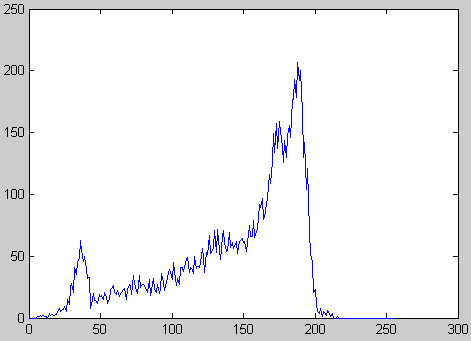
\includegraphics[width=\textwidth]{method_pics/orig.png}
  \caption{ВПИШИ подпись рисунку}
  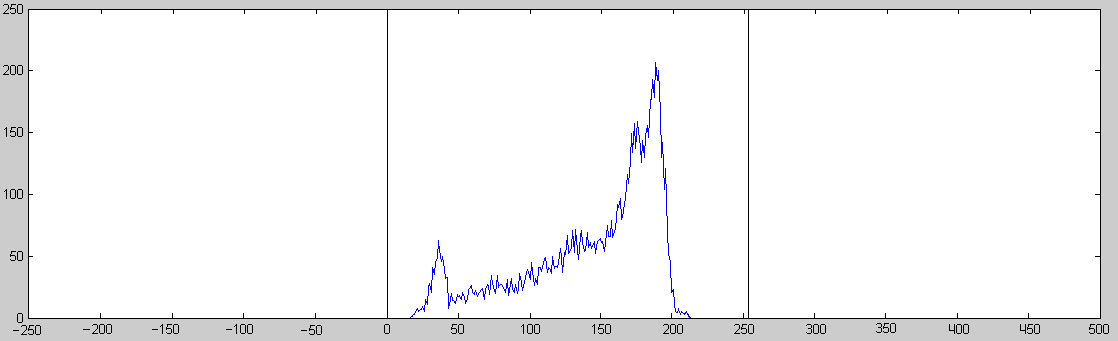
\includegraphics[width=\textwidth]{method_pics/wide.png}
  \caption{впиши подпись 2}
\end{figure}

Затем гистограмма тестируемого изображения будет перемещаться по эталонной гистограмме так, как это изображено на рисунках.

\begin{figure}[h]
  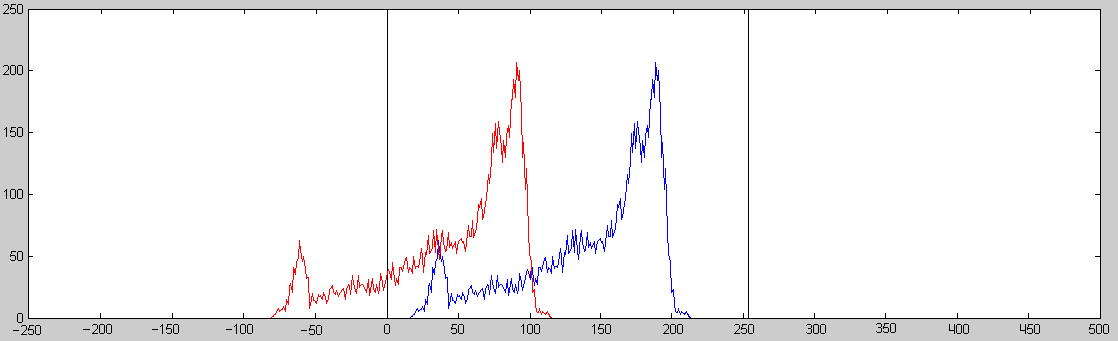
\includegraphics[width=\textwidth]{method_pics/wide+.png}
  \caption{ВПИШИ подпись рисунку}
  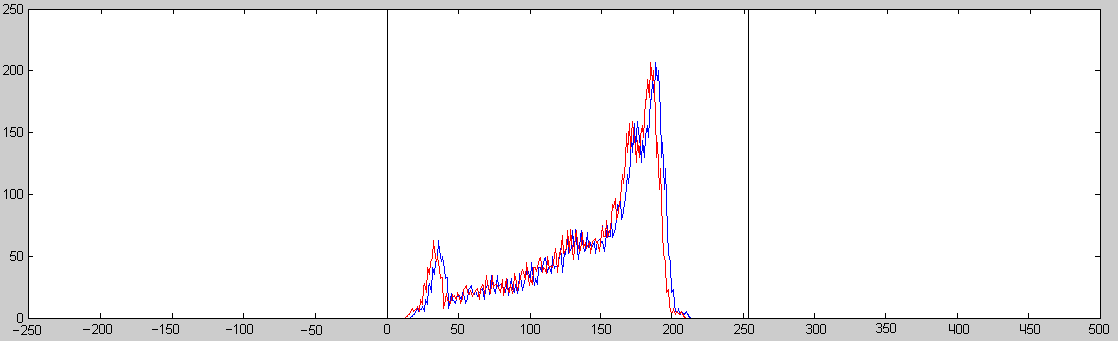
\includegraphics[width=\textwidth]{method_pics/wide++.png}
  \caption{впиши подпись 2}
\end{figure}

Каждый раз при наложении будет происходить расчёт метрики L2 отклонения между гистограммами базового и тестируемого изображений. За коэффициент соответствия между ними будет выбрано минимальное значение из всех подобных наложений. Далее, изображение, на котором наблюдался минимум из этих метрик, будет считаться распознанным тестовым изображением. При таком способе мы должны верно распознать не только похожие на тестируемое изображения, но и подвергшиеся изменению яркости.

\section*{Текст программ}
\addcontentsline{toc}{section}{Текст программ}

\lstinputlisting{./brightness_test/brightness_test.m}
\lstinputlisting{./editor_vs_matlab/editor_vs_matlab.m}
\lstinputlisting{./progs/colors.m}
\lstinputlisting{./progs/hist.m}
\lstinputlisting{./progs/hist2.m}
\lstinputlisting{./progs/light.m}

\section*{Результаты}
\addcontentsline{toc}{section}{Результаты}

\subsection*{Результаты работы на оригинальной базе ORL}
\addcontentsline{toc}{subsection}{Результаты работы на оригинальной базе ORL}

Ориганальная база содержит 40 классов по 10 изображений, из которых было взято 1 изображение в базу, 9 тестовых изображений.

\begin{tabular}{|c|c|c|}
\hline
              &  классический метод & модифицированный метод \\
\hline
32 столбца    &  58,6111            & 55,0000 \\
\hline
64 столбца    &  55,8333            & 53,3333 \\
\hline
128 столбцов  &  54,1667            & 52,5000 \\
\hline
256 столбцов  &  55,0000            & 52,2222 \\
\hline
\end{tabular}

Оригинальный метод демонстрирует распознавание примерно \textbf{55\%}, с отклонениями в пределах \textbf{3\%} 
в зависимости от размерности используемой гистограммы.
Модифицированный метод показывает распознавание на уровне \textbf{53\%} с отклонениями в \textbf{2\%}. 
Мы наблюдаем небольшое снижение распознавания около \textbf{2\%} за счёт неверной идентификации изображений с 
похожим характером гистограммы, но различным яркостным сдвигом.


\subsubsection*{40 классов, 2 изображения в базе, 8 тестовых изображений}

\begin{tabular}{|c|c|c|} \hline
& классический метод & модифицированный метод\\ \hline
32 столбца &66,5625&64,6875\\ \hline
64 столбца &63,1250&61,8750\\ \hline
128 столбцов&62,1875&60,9375\\ \hline
256 столбцов&63,1250&60,9375\\ \hline
\end{tabular}

Добавление второго тестового изображения ощутимо поднимает результативность классического метода (примерно до \textbf{64\%}
 с отклонением в \textbf{3\%}).
Модифицированный метод снова уступает с показателем в \textbf{62\%} и отклонением в \textbf{2\%}.

\subsection*{Результаты работы на модифицированной базе ORL}
\addcontentsline{toc}{subsection}{Результаты работы на модифицированной базе ORL}

\subsubsection*{40 классов, 1 изображение в базе, 9 тестовых изображений}

\begin{tabular}{|c|c|c|} \hline
&классический метод&модифицированный метод\\  \hline
32 столбца&23,6111&54,1667\\ \hline
64 столбца&23,0556&52,7778\\ \hline
128 столбцов&22,5000&52,7778\\ \hline
256 столбцов&23,0556&52,0000\\ \hline
\end{tabular}

На модифицированной базе впервые проявляется преимущество модифицированного метода. 
В то время как классический метод на осветлённых изображениях продемонстрировал 
показатели \textbf{23}$\pm$\textbf{2\%}, 
модифицированный смог удержать показатель на уровне \textbf{52}$\pm$\textbf{2\%}, 
то есть обеспечил более чем 2-кратное преимущество. Результат объясним, если вспомнить, что в данном тесте 
изображение в базе только (оригинал), что делает почти невозможным для классического метода распознавание 
осветлённых чётных по номерам изображений.

\subsubsection*{40 классов, 2 изображения в базе, 8 тестовых изображений}

\begin{tabular}{|c|c|c|} \hline
&классический метод&модифицированный метод\\ \hline
32 столбца&52,5000&62,5000\\ \hline
64 столбца&51,5625&60,9375\\ \hline
128 столбцов&49,6875&61,2500\\ \hline
256 столбцов&50,9375&61,2500\\ \hline
\end{tabular}

Теперь в базу входят 2 изображения, один оригинал и одно осветлённое, что должно уравнять шансы методов. 
Тем не менее, модифицированный метод с показателем \textbf{61}$\pm$\textbf{1\%} демонстрирует практически 
10-процентное преимущество над классическим с \textbf{51}$\pm$\textbf{2\%} распознавания.


\section*{Выводы}
\addcontentsline{toc}{section}{Выводы}

В ходе данного исследования была разработана модификация гистограммного метода, предназначенная для распознавания изображений различной степени яркости.

Достоинства модификации:
1. Более чем двукратное увеличение процента распознавания (по сравнению с оригинальным методом) на базах, содержащих различные по яркости изображения, в случае использования одного тестового изображения в базе.
2. 10-типроцентное увеличение процента распознавания (по сравнению с оригинальным методом) при использовании двух тестовых изображений в базе.

Недостатки модификации:
1. Замедление работы в 2*K раз (по сравнению с оригинальным методом), где K - количество отсчётов гистограммы (255 в нашем исследовании)
2. Ухудшение распознавания порядка 2\% по сравнению с оригинальным методом - на базах, все изображения в которых имеют относительно небольшие отклонения по яркости (причина в неверной идентификации изображений со схожим характером гистограммы, но различным яркостным сдвигом).

Основным направлением для дальнейшей работы видится улучшение производительности метода, т.к. на текущий момент его трудоёмкость достаточно высока.

Данную модификацию можно применять в системах автоматического видео наблюдения, установленных в условиях сложной освещенности, например,
уличные банкоматы или автоматичесские системы наблюдения за дорожной обстановкой.  

\section*{Список литературы}

\addcontentsline{toc}{section}{Список литературы}


\begin{enum}
\item
Кухарев\,Г.\,А. Биометрические системы: Методы и средства идентификации личности человека. --- СПб.: Политехника, 2001.
\item
Журнал о безопастности бизнеса и личности <<БДИ>>, \No 5 2004 г. ; \No 3 2005 г.
\end{enum}

\end{document}


